\section{Transformer Model} \label{Transformer}

\begin{figure}[h]
\vspace{-10pt}
\centering
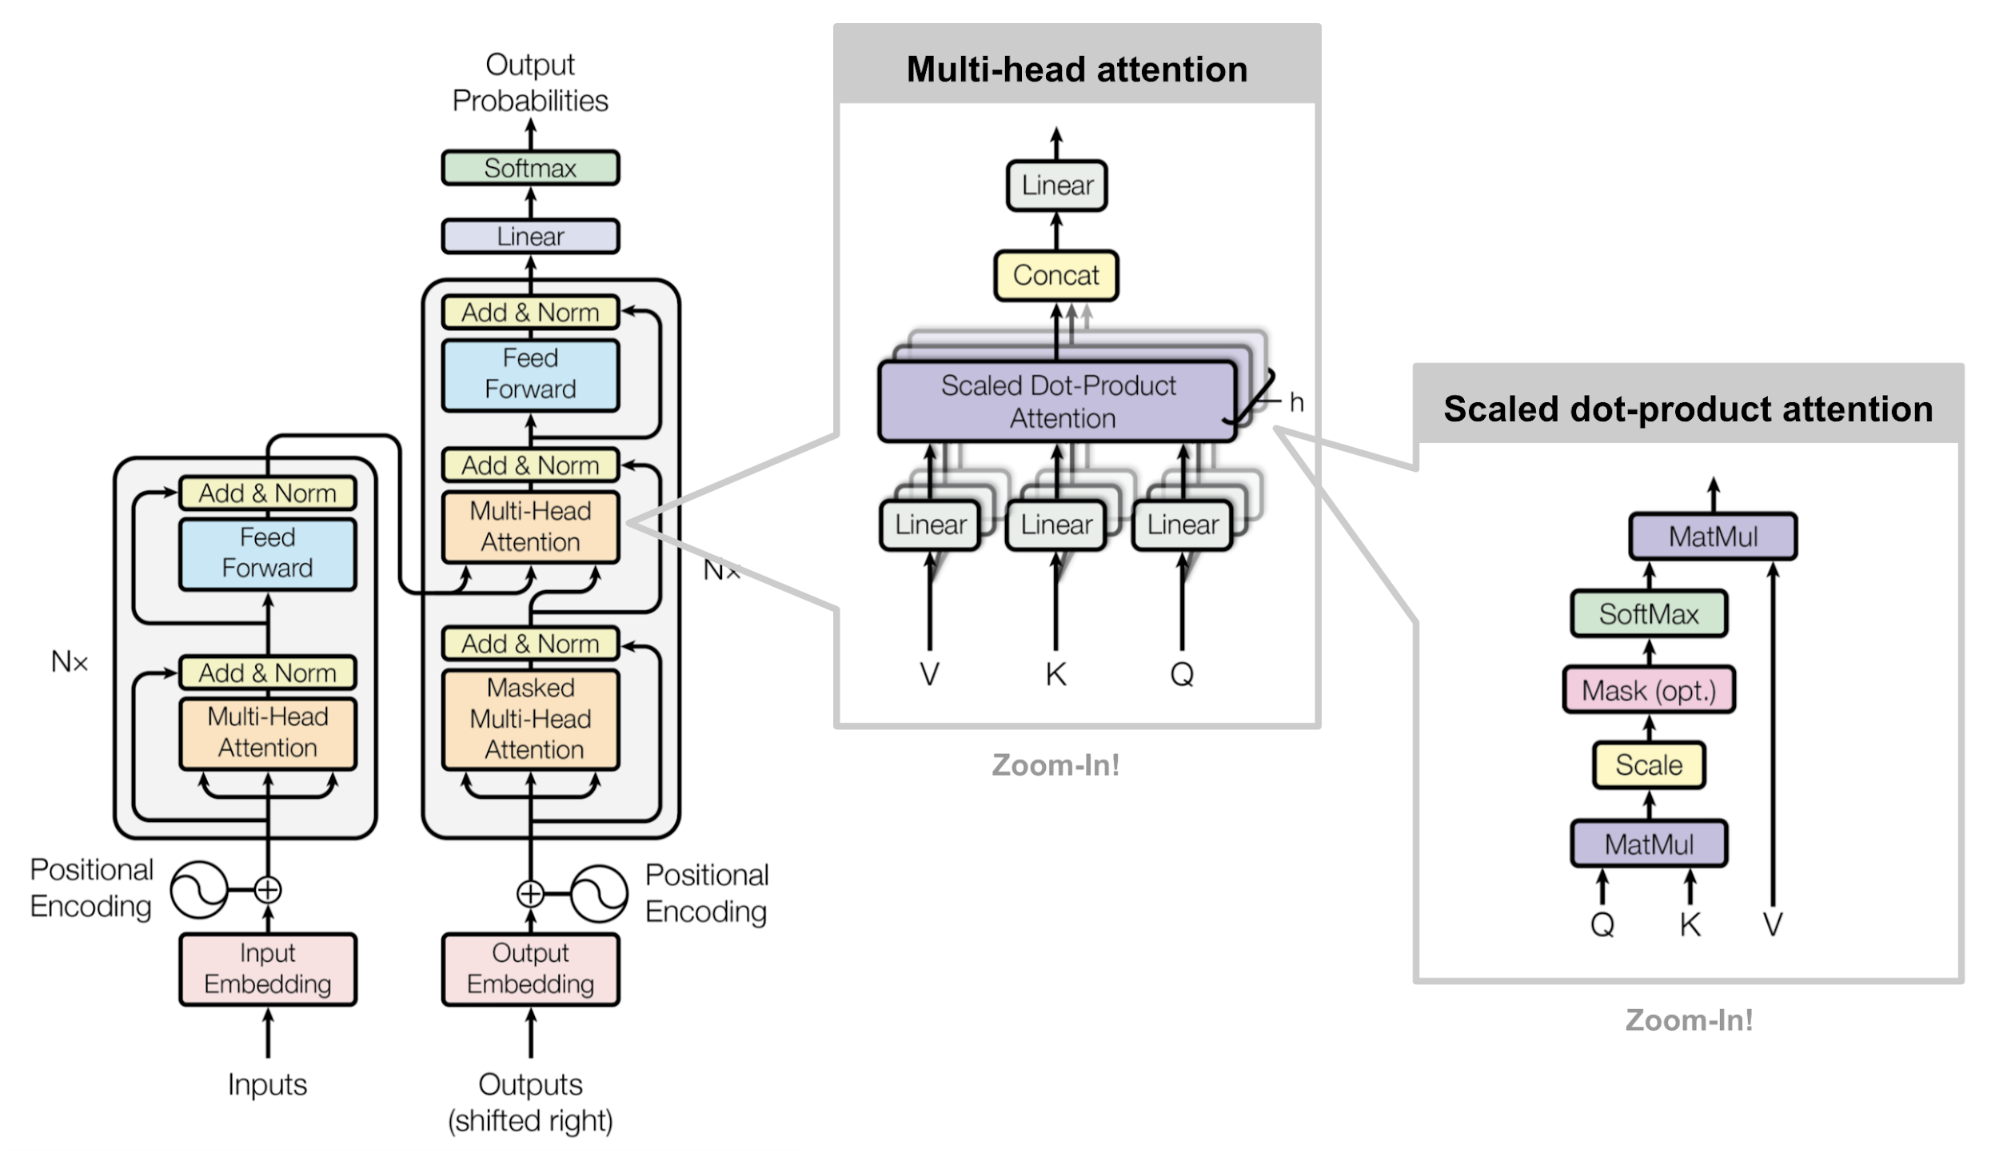
\includegraphics[width=0.95\textwidth]{imgs/transformer.png}
\vspace{-10pt}
\caption{\footnotesize Transformer model architecture. The gray boxes hold Encoder and Decoder layers, respectively, which are each repeated $N=6$ times. From \emph{Attention? Attention}, by Weng, 2018. \url{https://lilianweng.github.io/lil-log/2018/06/24/attention-attention.html}. Copyright 2018 by Weng.}
\vspace{-5pt}
\end{figure}

The \textbf{Transformer model} introduced by Vaswani et al. (2017) is a neural machine translation (NMT) model that proves more parallelizable than seq-to-seq models with attention. Rather than using recurrent neural networks (RNNs) combined with the \textbf{attention mechanism}, the Transformer sequence-to-sequence model uses only a \textbf{self attention mechanism} to attend to different word tokens in an input sentence and thus generate a sequence of contextual embeddings. 




\subsection{Encoder}

The Encoder is a \textbf{bidirectional recurrent network (RNN)} consisting of a forward RNN and backward RNN. The forward RNN reads the input sequence $\overrightarrow{x} = \Big\{ x_1,...,x_{T_x} \Big\}$ from left to right to produce a sequence of forward hidden states $\Big\{ \overrightarrow{h_1},..., \overrightarrow{h_{T_x}} \Big\}$. The backward RNN reads the sequence in reverse order, so taking $x_{T_x}$ to $x_1$ and returns a sequence of backward hidden states $\Big\{ \overleftarrow{h_1},..., \overleftarrow{h_{T_x}} \Big\}$. Then, for each word $x_t$ an annotation is obtained by concatenating the corresponding forward hidden state vector $\overrightarrow{h}_t$ with the backward one $\overleftarrow{h}_t$, such that $h_t = \Big \{ \overrightarrow{h}_t^T \; ; \; \overleftarrow{h}_t^T \Big\}^T , \: t=1,...,T_x$. This allows the annotation vector $h_t$ for word $x_t$ to contain contextual information by using previous and latter words (Bahdanau et al., 2016). These annotations are later used in the decoder to compute the context vector. 

The Encoder is composed of $N$ identical \textbf{Encoder layers}, which together are named the \textbf{Encoder stack}. A single \textbf{Encoder layer}  is composed of two sub-layers: 
\begin{enumerate}
    \item \textbf{multi-head self attention mechanism (layer)}
    
    \item \textbf{positionwise fully-connected feed-forward network (layer)}
\end{enumerate}

A \textbf{residual connection layer} surrounds each of these sub-layers, and this is followed by \textbf{layer normalization} (Trevett, 2020).  



\subsection{Decoder}


The Decoder neural network generates hidden states $s_t = \text{Decoder}\Big( s_{t-1}, y_{t-1}, c_t \Big)$ for time steps $t = 1,..., m$ where the context vector $c_t = \sum_{i=1}^n \alpha_{ti} \cdot h_i$ is a sum of the hidden states of the input sentence, weighted by alignment scores, as for the Seq-to-Seq model (Weng, 2018). (Here the arrows denote the direction of the network rather than vector notation.)

Similarly to the Encoder, the Decoder contains a stack of $N$ Decoder layers which consist of several sub-layers:
\begin{enumerate}
    \item \textbf{multi-head self attention layer}
    \item \textbf{encoder-decoder attention layer} or masked multi-head attention. 
    
    \item \textbf{positionwise fully-connected feed forward layer}. 
\end{enumerate}

Like in the Encoder, in between each of these layers is a residual connection followed by layer normalization. 

\begin{figure}[h]
\vspace{-10pt}
\centering
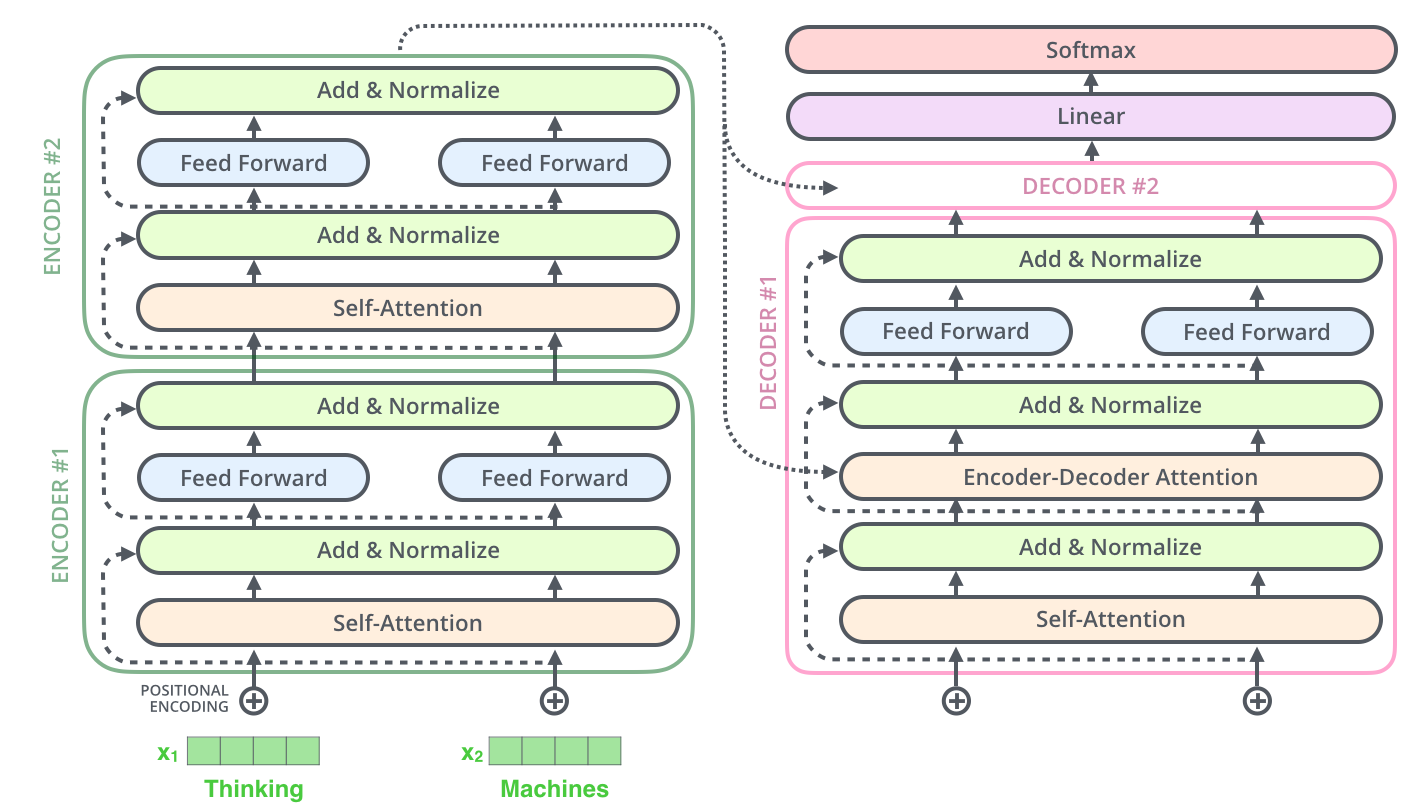
\includegraphics[width=0.8\textwidth]{imgs/encoderDecoderLayersDetailed.png}
\vspace{-10pt}
\caption{\footnotesize The layers inside Encoder and Decoder. From \emph{The Illustrated Transformer}, by Alammar, 2018. \url{https://jalammar.github.io/illustrated-transformer/}. Copyright 2018 by Alammar.}
\vspace{-5pt}
\end{figure}



\subsection{Self-Attention}

\subsubsection{Motivation for Self-Attention}

Consider the following sentence: 


\begin{shadequote}{}
\vspace{10pt}
\Large \textit{The animal didn't cross the road because it was too tired.}
\vspace{10pt}
\end{shadequote}

What does ``it” in this sentence refer to? Is ``it" referring to the street or to the animal? This question may be simple to a human but not to a machine. 

This is the motivation for \textbf{self-attention}: when the Transformer processes the word ``it", self-attention allows it to associate ``it" with ``animal". As the Transformer processes each word, self-attention allows it to look at other positions in the input sentence for clues to create a better encoding for this word. In each layer, a part of the attention mechanism that focuses on ``the animal" was \emph{baked in} to a part of the representation of the word ``it" when encoding this in the model (Trevett, 2020). 


\subsubsection{Query, Key, Value}

Formally, ``an attention function can be described as mapping a query and a set of key-value pairs to an output, where the \textbf{query, keys, values}, and output are all vectors. The output is computed as a weighted sum of the values, where the weight assigned to each value is computed by a compatibility function of the query with the corresponding key" (Vaswani et al., 2017). 


The \textbf{query, key, and value} vectors are abstractions useful for calculating attention:
\begin{itemize}
    \item The Query matrix $Q$ contains information on which word to calculate self attention. 
    
     \item The Key matrix $K$ contains vector information for \emph{each} word in the sentence.
     
    \item The Value matrix $V$ contains vector information for the rest of the words in the sentence. Multiplying the query vector with the key vector of a particular word, stored in $Q$ and $K$ computes a result that indicates how much \emph{value} vector $V$ to consider.
\end{itemize}

For the previous sentence, ``The animal didn't cross the street because it was too tired,"  $Q$ query refers to the word ``it"; $V$ contains vectors for words other than ``it"; $K$ contains vectors for each word, including ``it".

The final embedding of the word or \textbf{output} is a weighted sum of \textbf{value} vectors and softmax probabilities of the dot product between query and key vectors: 
$$
Attention \Big(Q, K, V \Big) = softmax \Bigg(\frac {QK^T} {\sqrt{d_k}} \Bigg) V
$$
Each word has an associated \textbf{query, key, value} vector which are created by multiplying the words embeddings with parameter weight matrices $W^Q, W^K, W^V$ that are associated with the query, key, and value matrices, respectively. For the example sentence, let the input be the matrix $X = \{\overrightarrow{x_1}, \overrightarrow{x_2}, ..., \overrightarrow{x_n}\}$ for where vector $\overrightarrow{x_i}$ corresponds to word $i$, and there are $n$ words. Then the input word vectors are: 
% $
% \overrightarrow{x_1} = \text{"The"}, \!
% \overrightarrow{x_2} = \text{"animal"}, \!
% \overrightarrow{x_3} = \text{"didn't"}, \!
% \overrightarrow{x_4} = \text{"cross"}, \!
% \overrightarrow{x_5} = \text{"the"}, \!
% \overrightarrow{x_6} = \text{"street"}, \!
% \overrightarrow{x_7} = \text{because"}, \!
% \overrightarrow{x_8} = \text{"it"}, \!
% \overrightarrow{x_9} = \text{"was"}, \!
% \overrightarrow{x_{10}} = \text{"too"}, \!
% \overrightarrow{x_{11}} = \text{"tired"}, \!
% \overrightarrow{x_{12}} = "." 
% $

$$
\begin{array}{ll}
\overrightarrow{x_1} = \text{"The"} \\
\overrightarrow{x_2} = \text{"animal"} \\
\overrightarrow{x_3} = \text{"didn't"} \\
\overrightarrow{x_4} = \text{"cross"} \\
\overrightarrow{x_5} = \text{"the"} \\
\overrightarrow{x_6} = \text{"street"} \\
\overrightarrow{x_7} = \text{because"} \\
\overrightarrow{x_8} = \text{"it"} \\
\overrightarrow{x_9} = \text{"was"} \\
\overrightarrow{x_{10}} = \text{"too"} \\
\overrightarrow{x_{11}} = \text{"tired"} \\
\overrightarrow{x_{12}} = "." \\
\end{array}
$$
and the word embedding vectors would be denoted $\Big\{ \overrightarrow{w_1}, \overrightarrow{w_2}, ..., \overrightarrow{w_n} \Big\}$ and the $n$ \textbf{query, key, value} vectors for each word are denoted $\Big\{\overrightarrow{q_1}, \overrightarrow{q_2}, ..., \overrightarrow{q_n} \Big\}$, $\Big\{\overrightarrow{k_1}, \overrightarrow{k_2}, ..., \overrightarrow{k_n} \Big\}$, $\Big\{\overrightarrow{v_1}, \overrightarrow{v_2}, ..., \overrightarrow{v_n} \Big\}$ respectively.


\subsubsection{Self-Attention: Vector Calculation}

\underline{Step 1: Create Query, Key, Value Vectors}

The first step is to create three vectors from each of the Encoder's input vectors (in this case, the inputs are the embeddings $\overrightarrow{w_i}$ of each word $\overrightarrow{x_i}$). So for each word, we create a Query vector, a Key vector and a Value vector by multiplying the embedding by three matrices obtained during training
TODO: training matrices? to create Q, K, V
- NOTE: the embeddings $\overrightarrow{w_i}$ and `Encoder` input and output vectors have dimension $512$.
- NOTE: the query, key, value vectors have dimension $64$. These do not HAVE to be smaller, but this is just an architecture choice to make the computation of multiheaded attention (mostly) constant.
%% codecell
%% codecell
ImageResizer.resize(filename = pth + "qkv.png")
%% markdown [markdown]

Step 2: Calculate a Score
Say we are calculating the self-attention for word $i$ in this example, $\overrightarrow{x_i}$, whose numericalized word embedding is $\overrightarrow{w_i}$. We need to score each word of the input sentence against this word. The score determines how much **focus to place on other parts of the input sentence** as we encode a word at a certain position.

The score is calculated by taking the dot product of the *query* vector with the *key* vector of the respective word we are scoring. This means if we are processing the self-attention for the word in position $i$ (word $i$), the first value in the $i$th score vector would be the dot product of $\overrightarrow{q_i}$ and $\overrightarrow{k_1}$.

* the first score value in the $i$th score vector would be the dot product of $\overrightarrow{q_i}$ and $\overrightarrow{k_1}$.
* the second score value in the $i$th score vector would be the dot product of $\overrightarrow{q_i}$ and $\overrightarrow{k_2}$.
* the third score value in the $i$th score vector is is the dot product of $\overrightarrow{q_i}$ and $\overrightarrow{k_3}. $

$$ \vdots \\ $$
- the $n$-th score for the $n$-th word would be the dot product of $\overrightarrow{q_i}$ and $\overrightarrow{k_n}$.

$$
scores_{w_i} = \bigg\{
\overrightarrow{q_i} \cdot \overrightarrow{k_1},
\overrightarrow{q_i} \cdot \overrightarrow{k_2},
...,
\overrightarrow{q_i} \cdot \overrightarrow{k_n} \bigg\}
$$

The image below shows the first and second values in the first scoring vector corresponding to the first word "Thinking" in a sentence that starts with the words "Thinking Machines ...":
%% codecell
%% codecell
%% codecell

%% markdown [markdown]

Step 3: Scale The Score

The dimensions of the  key vectors is $d_k = 64$.

From the paper:
> *We suspect that for large values of $d_k$, the dot products grow large in  magnitude, pushing the `softmax function` into regions where it has extremely small gradients. To counteract this effect, we scale the dot products by $\frac {1} {\sqrt{d_k}}$*

So now the scores vector for the first `word embedding` `tensor` $\overrightarrow{w_i}$ is:

$$
scores_{w_i} = \Bigg\{
\frac {\overrightarrow{q_i} \cdot \overrightarrow{k_1}} {\sqrt{d_k}},
\frac {\overrightarrow{q_i} \cdot \overrightarrow{k_2}} {\sqrt{d_k}},
...,
\frac{\overrightarrow{q_i} \cdot \overrightarrow{k_n}} {\sqrt{d_k}} \Bigg\}
$$


Step 4: Apply Softmax

The softmax function normalizes the scores so they become positive and add up to $1$. This serves the purpose that now the scores are a probability distribution.
$$
scores_{w_i} = softmax \Bigg( \Bigg\{
\frac {\overrightarrow{q_i} \cdot \overrightarrow{k_1}} {\sqrt{d_k}},
\frac {\overrightarrow{q_i} \cdot \overrightarrow{k_2}} {\sqrt{d_k}},
...,
\frac{\overrightarrow{q_i} \cdot \overrightarrow{k_n}} {\sqrt{d_k}} \Bigg\} \Bigg)
$$

The image below shows the scaling and softmax operations after the query, key, value operations:

%% codecell
Image(filename = pth + "scaling.png")
%% markdown [markdown]

Step 5: Compute the Weights

Multiply each *value vector* contained in the value matrix $V$ by the softmax scores. The intuition is to keep intact the values of the words we must focus on and drown out irrelevant words. This is why we weight the value vector by the softmax scores.
$$
weightedValues_{w_i} = scores_{w_i} * (\overrightarrow{v_1}, ..., \overrightarrow{v_n})
$$


Step 6: Output Vector

Sum up the weighted value vectors to produce the **output vector** of the self-attention layer of the current first word $\overrightarrow{w_i}$.
$$
\overrightarrow{output_{w_i}} = softmax \Bigg(
\frac {\overrightarrow{q_i} \cdot \overrightarrow{k_1}} {\sqrt{d_k}} \Bigg) \cdot \overrightarrow{v_1} +
softmax \Bigg(\frac {\overrightarrow{q_i} \cdot \overrightarrow{k_1}} {\sqrt{d_k}} \Bigg) \cdot \overrightarrow{v_2} + ... +
softmax \Bigg(\frac {\overrightarrow{q_i} \cdot \overrightarrow{k_1}} {\sqrt{d_k}} \Bigg) \cdot \overrightarrow{v_n}
$$

The image below shows the last step 5 and step 6:
%% codecell
%% codecell
%% codecell

\subsection{Multi-Head Attention}

\subsubsection{Motivation for Multi-Head Attention}

\subsubsection{Multi-Head Attention: Matrix Calculation}

\subsection{Encoder-Decoder Attention}

\subsection{Positional Encodings}

\subsection{Position-wise Feed Forward Layer}

\subsection{Residual Connection}

\subsection{Layer Normalization}


\subsection{Transformer Workflow}